\documentclass[12pt]{article}

\usepackage{sbc-template}
\usepackage{graphicx,url}
\usepackage[utf8]{inputenc}
\usepackage[brazil]{babel}
\usepackage{amsmath}
\usepackage{amsfonts}

\sloppy

\title{Análise Comparativa de Estruturas Disjoint Set Union:\\Impacto das Heurísticas de Otimização no Algoritmo de Kruskal}

\author{Enzo Barcelos\inst{1}}

\address{Curso de Engenharia de Software -- Pontifícia Universidade Católica de Minas Gerais (PUC Minas)
  \email{enzo.barcelos@sga.pucminas.br}
}

\begin{document}

\maketitle

\begin{resumo}
  Este trabalho analisa experimentalmente três variantes da estrutura Disjoint Set Union (DSU) aplicadas ao algoritmo de Kruskal para o cálculo de Árvores Geradoras Mínimas: a implementação Ingênua, Union by Rank e a versão completa de Tarjan (Union by Rank com Path Compression). Os experimentos foram realizados em grafos conexos aleatórios com $n$ entre $10^3$ e $10^5$ vértices e $m = 3n$ arestas, medindo tempo de execução e número de acessos ao array de pais. As medições reportadas são médias sobre cinco grafos distintos por configuração, acompanhadas do desvio padrão amostral nos tempos. Os resultados evidenciam na prática a transição entre as classes $O(n)$, $O(\log n)$ e $O(\alpha(n))$: a versão Ingênua ultrapassa $8 \times 10^9$ acessos e aproximadamente 16 segundos em $n = 10^5$, enquanto Tarjan mantém o custo médio por aresta essencialmente constante, com redução de mais de três ordens de grandeza. Com a estrutura de Tarjan, o custo do DSU deixa de influenciar o tempo total do Kruskal, que passa a ser dominado pela ordenação das arestas.
\end{resumo}

\begin{abstract}
  This paper presents an experimental analysis of three Disjoint Set Union (DSU) variants applied to Kruskal's Minimum Spanning Tree algorithm: Naive, Union by Rank, and Full Tarjan (Union by Rank combined with Path Compression). Experiments were conducted on randomly generated connected graphs with $n$ ranging from $10^3$ to $10^5$ vertices and $m = 3n$ edges, measuring both execution time and array-access counts. Each data point is the mean over five distinct graphs, with sample standard deviation reported for timings. Results show a clear practical transition across complexity classes $O(n)$, $O(\log n)$, and $O(\alpha(n))$: the Naive implementation reaches over $8 \times 10^9$ accesses and around 16 seconds at $n = 10^5$, while Tarjan keeps the per-edge cost essentially constant, reducing accesses by more than three orders of magnitude. Under Tarjan's structure, the dominant cost in Kruskal shifts entirely to edge sorting, confirming that the DSU overhead becomes negligible in practice.
\end{abstract}

\noindent\textbf{Palavras-chave:} Union-Find; Disjoint Set Union; Algoritmo de Kruskal; Path Compression; Complexidade Amortizada; Função Inversa de Ackermann.


\section{Introdução}

Gerenciar conjuntos disjuntos é um problema recorrente em computação. Aparece no processamento de imagens, quando pixels vizinhos precisam ser agrupados em regiões. Aparece em redes, quando se quer saber se dois nós pertencem à mesma componente conectada. E aparece, talvez da forma mais explícita, em algoritmos de grafos que testam conectividade dinamicamente.

A estrutura de dados conhecida como \textit{Disjoint Set Union} (DSU), ou simplesmente \textit{Union-Find}, foi projetada para resolver esse problema de forma eficiente. Ela mantém uma coleção de conjuntos disjuntos e oferece duas operações fundamentais: \texttt{Find}, que identifica a qual conjunto um elemento pertence, e \texttt{Union}, que funde dois conjuntos em um só.

Uma implementação simples dessa estrutura, utilizando árvores sem nenhum critério de balanceamento, pode levar a cadeias longas de ponteiros, degradando o desempenho das operações para $O(n)$ no pior caso. Robert Tarjan propôs duas heurísticas que, quando combinadas, reduzem a complexidade amortizada para $O(\alpha(n))$, onde $\alpha$ é a inversa da função de Ackermann. Essa função cresce tão lentamente que, para qualquer valor prático de $n$, seu resultado não ultrapassa 4 \cite{tarjan1975}.

O presente trabalho implementa três variantes do DSU com níveis crescentes de otimização e avalia experimentalmente o impacto no desempenho do algoritmo de Kruskal para Árvores Geradoras Mínimas (MST). Duas questões orientam a análise: (i) a partir de qual escala a implementação ingênua deixa de ser viável em aplicações reais de MST? e (ii) qual o ganho marginal efetivo da combinação de Union by Rank com Path Compression em relação ao uso isolado de Union by Rank?

A contribuição do trabalho é empírica: as três variantes foram implementadas em Java com instrumentação de contadores de acesso a memória, e os resultados são apresentados tanto em escala linear quanto logarítmica, incluindo uma análise de expoente empírico que quantifica as classes de complexidade observadas. O Algoritmo de Kruskal foi escolhido como ambiente de teste por exercitar, por construção, sequências intercaladas de \texttt{Find} e \texttt{Union} na proporção $\Theta(m)$, cenário que expõe com clareza as diferenças entre as variantes.

O restante do artigo está organizado da seguinte forma: a Seção~\ref{sec:fundamentacao} apresenta a fundamentação teórica; a Seção~\ref{sec:metodologia} descreve a metodologia e o ambiente experimental; a Seção~\ref{sec:resultados} discute os resultados obtidos; e a Seção~\ref{sec:conclusao} conclui o trabalho.


\section{Fundamentação Teórica}
\label{sec:fundamentacao}

\subsection{A Estrutura Disjoint Set Union}

A estrutura DSU representa cada conjunto como uma árvore enraizada. Cada elemento possui um ponteiro para seu pai, e a raiz de cada árvore serve como representante do conjunto. Inicialmente, cada elemento é seu próprio pai, formando $n$ conjuntos unitários.

A operação \texttt{Find(x)} percorre a cadeia de ponteiros a partir de $x$ até encontrar a raiz, ou seja, o elemento cuja referência aponta para si mesmo. A operação \texttt{Union(x, y)} localiza as raízes dos conjuntos de $x$ e $y$ e, caso sejam diferentes, faz a raiz de um apontar para a raiz do outro.

\subsection{Implementação Ingênua}

Na versão mais simples, o \texttt{Union} conecta uma raiz à outra sem nenhum critério de escolha. O problema dessa abordagem é que, em sequências adversas de operações, a árvore pode degenerar em uma lista encadeada. Nesse cenário, cada chamada a \texttt{Find} precisa percorrer até $n$ ponteiros, resultando em complexidade $O(n)$ por operação.

\subsection{Union by Rank}

A heurística de \textit{Union by Rank} busca manter as árvores balanceadas. Cada nó mantém um valor de \textit{rank}, que funciona como um limitante superior da altura da subárvore. Na união de dois conjuntos, a raiz com menor \textit{rank} é pendurada sob a raiz com maior \textit{rank}. Quando ambos têm o mesmo \textit{rank}, escolhe-se uma arbitrariamente e incrementa-se seu \textit{rank}.

Essa estratégia garante que a altura de qualquer árvore com $k$ elementos não ultrapasse $\lfloor \log_2 k \rfloor$. Isso ocorre porque, para que uma árvore atinja \textit{rank} $r$, ela precisa ter sido unida com outra árvore de \textit{rank} $r-1$, o que exige ao menos $2^r$ elementos. Portanto, a complexidade do \texttt{Find} fica limitada a $O(\log n)$.

\subsection{Path Compression}

A heurística de \textit{Path Compression} modifica a operação \texttt{Find} para que, ao percorrer o caminho até a raiz, todos os nós visitados passem a apontar diretamente para ela. Isso ``achata'' a árvore progressivamente, tornando consultas futuras sobre os mesmos elementos praticamente instantâneas.

Usada isoladamente, sem Union by Rank, Path Compression garante complexidade amortizada $O(\log n)$ por operação \cite{tarjan1975}, com pior caso $O(n)$ em chamadas individuais. O ganho expressivo vem justamente da combinação: árvores com altura limitada por $O(\log n)$ (via Rank) e compressão progressiva desse caminho curto (via PC) resulta na complexidade amortizada $O(\alpha(n))$, que é o tema da seção seguinte.

\subsection{A Complexidade $O(\alpha(n))$ de Tarjan}

Para entender por que a combinação de Union by Rank e Path Compression produz complexidade amortizada $O(\alpha(n))$, é preciso distinguir custo real de custo amortizado. A análise amortizada distribui o custo total de uma sequência de operações uniformemente entre elas: mesmo que uma operação individual seja cara, o custo médio por operação ao longo da sequência pode ser muito menor.

Tarjan provou esse resultado usando o \textit{método do potencial} \cite{tarjan1985}: associa-se a cada nó uma função de potencial que depende do seu rank e de sua posição na árvore. Operações de \texttt{Find} que percorrem caminhos longos reduzem o potencial ao comprimir nós, de modo que seu custo real alto é compensado por uma queda equivalente no potencial. O custo amortizado por operação (custo real somado à variação de potencial) fica limitado a $O(\alpha(n))$.

O resultado formal é o seguinte: qualquer sequência de $m$ operações sobre $n$ elementos tem custo total $O((m + n) \cdot \alpha(n))$, onde $\alpha$ é a inversa da função de Ackermann \cite{tarjan1975,tarjan1984}.

A função de Ackermann $A(k, j)$ é definida recursivamente como \cite{cormen2009}:
\begin{align}
A(1, j) &= 2^j, \quad \text{para } j \geq 1 \\
A(k, 1) &= A(k-1, 2), \quad \text{para } k \geq 2 \\
A(k, j) &= A(k-1, A(k, j-1)), \quad \text{para } k \geq 2, j \geq 2
\end{align}

Essa função cresce de forma super-exponencial. $A(4, 1)$, por exemplo, supera uma torre de potências de 2 com $2^{16} = 65.536$ andares. Sua inversa $\alpha(n) = \min\{k \geq 1 : A(k, 1) \geq n\}$ cresce com a mesma lentidão, agora para o lado oposto. Para qualquer $n$ imaginável no universo físico, $\alpha(n) \leq 4$ \cite{cormen2009}. Formalmente a complexidade não é $O(1)$; na prática, é constante.

A Tabela~\ref{tab:alpha} ilustra essa propriedade com valores concretos.

\begin{table}[!ht]
\centering
\caption{Valores de $\alpha(n)$ para diferentes ordens de grandeza de $n$}
\label{tab:alpha}
\begin{tabular}{|r|c|}
\hline
\textbf{$n$} & \textbf{$\alpha(n)$} \\
\hline
$\leq 2$ & 1 \\
$\leq 2^4 = 16$ & 2 \\
$\leq 2^{65536}$ & 3 \\
$\leq A(4,1)$ (número com $10^{19728}$ dígitos) & 4 \\
\hline
\end{tabular}
\end{table}

\subsection{O Algoritmo de Kruskal}

O algoritmo de Kruskal resolve o problema da Árvore Geradora Mínima (MST) para grafos conexos ponderados \cite{kruskal1956}. Seu funcionamento é direto: ordena todas as arestas do grafo por peso crescente e percorre essa lista, adicionando cada aresta à MST se ela não formar ciclo com as arestas já selecionadas \cite{sedgewick2011}. A detecção de ciclos é feita verificando se os dois vértices da aresta pertencem ao mesmo conjunto, o que é exatamente o que o DSU oferece.

A complexidade total do Kruskal é $O(m \log m)$ para a ordenação das arestas somada ao custo das operações de \texttt{Find} e \texttt{Union}. Com o DSU de Tarjan, essas operações têm custo amortizado $O(\alpha(n))$ cada, totalizando $O(m \cdot \alpha(n))$ para a parte de conjuntos disjuntos, o que na prática não adiciona overhead significativo além da ordenação.


\section{Metodologia}
\label{sec:metodologia}

\subsection{Escolhas de Modularização}

O projeto foi desenvolvido em Java e organizado em três pacotes, cada um com responsabilidade bem definida:

\begin{itemize}
  \item \textbf{Pacote \texttt{dsu}}: Contém uma interface \texttt{DSU} que define o contrato das operações (\texttt{find}, \texttt{union}, \texttt{makeSet}) e um método \texttt{getContador()} para contagem de acessos. As três variantes (\texttt{DSUNaive}, \texttt{DSURank} e \texttt{DSUTarjan}) implementam essa interface.

  \item \textbf{Pacote \texttt{grafo}}: Contém a classe \texttt{Aresta} (com atributos \texttt{u}, \texttt{v}, \texttt{peso} e implementação de \texttt{Comparable}) e a classe \texttt{Kruskal}, que recebe qualquer objeto do tipo \texttt{DSU} por polimorfismo.

  \item \textbf{Pacote \texttt{benchmark}}: Contém a classe responsável por gerar grafos aleatórios, executar o Kruskal com cada variante e medir os resultados.
\end{itemize}

A vantagem dessa divisão é prática: uma nova variante de DSU entra no experimento criando-se uma classe que implemente a interface e passando-a ao Kruskal. Nenhum outro arquivo precisa mudar. Como consequência secundária, grafo e DSU podem ser testados em isolamento.

\subsection{Implementação das Variantes}

Cada variante do DSU mantém um contador interno que registra o total de acessos ao array \texttt{pai[]}: cada leitura usada para comparação ou avanço de ponteiro conta como 1 acesso; cada escrita (union ou compressão de caminho) também conta como 1. A política é uniforme entre as três variantes, conforme documentado na interface \texttt{DSU.java}, o que permite comparação direta independente de variações de tempo causadas pelo sistema operacional ou escalonamento de processos.

\begin{itemize}
  \item \textbf{DSUNaive}: Utiliza apenas o array \texttt{pai[]}. O \texttt{find} percorre a cadeia até a raiz sem modificá-la. O \texttt{union} simplesmente conecta uma raiz à outra.

  \item \textbf{DSURank}: Adiciona o array \texttt{rank[]}. O \texttt{find} permanece sem compressão. O \texttt{union} compara os \textit{ranks} e pendura a árvore menor sob a maior.

  \item \textbf{DSUTarjan}: Combina \texttt{rank[]} com compressão de caminho no \texttt{find}. A implementação é recursiva: cada chamada faz o nó visitado apontar diretamente para a raiz retornada.
\end{itemize}

\subsection{Validação de Correção}

Antes dos experimentos de desempenho, verificou-se que as três variantes produzem exatamente o mesmo peso total de MST para cada grafo de teste. O método \texttt{Main.exemploKruskal()} executa essa verificação num grafo de 6 vértices com solução conhecida e lança \texttt{AssertionError} caso qualquer variante divirja das demais (tolerância de $10^{-9}$). A consistência dos pesos confirma que as otimizações não alteram a correção do algoritmo.

\subsection{Geração de Grafos de Teste}

Para cada tamanho $n$, foram gerados grafos com $m = 3n$ arestas. A geração garante conectividade construindo primeiro uma árvore geradora (cada vértice $i$ é conectado a um vértice aleatório $j < i$) e então adicionando $m - (n-1)$ arestas extras aleatórias. Os pesos são valores reais uniformemente distribuídos no intervalo $[0, 100)$.

Em cada configuração foram usadas cinco seeds fixas (de 42 a 46), gerando cinco grafos distintos. Dentro de um mesmo grafo, as três variantes processam exatamente a mesma sequência de arestas, de modo que a comparação de contagens e tempos é sempre feita sobre dados idênticos. A ordenação das arestas é feita por \texttt{Collections.sort()}, que usa o algoritmo Timsort com complexidade $O(m \log m)$.

Algumas limitações do gerador merecem registro: self-loops ($u = v$) são descartados sem reposição, de modo que o número efetivo de arestas pode ser levemente inferior a $3n$; arestas duplicadas são permitidas; e a topologia do grafo é enviesada para o padrão ``árvore-caminho com arestas extras'', não representando a distribuição uniforme de um grafo de Erd\H{o}s--R\'enyi.

\subsection{Cenários de Teste}

Os testes foram realizados para cinco tamanhos de entrada: $n \in \{1.000;\; 5.000;\; 10.000;\; 50.000;\; 100.000\}$. Para cada configuração, o Kruskal foi executado com as três variantes de DSU em cinco grafos distintos, gerados com as seeds $42$, $43$, $44$, $45$ e $46$. Em cada execução foram medidos o tempo via \texttt{System.nanoTime()} e a contagem de acessos ao array de pais. Os valores reportados nas tabelas são a média das cinco repetições; para os tempos, também se reporta o desvio padrão amostral.

\subsection{Ambiente de Execução}

Os experimentos foram conduzidos no seguinte ambiente:

\begin{itemize}
  \item \textbf{Sistema Operacional}: Windows 11 Pro (Build 26200)
  \item \textbf{Processador}: Intel Core i7-13650HX (16 núcleos, clock base 2,6 GHz, boost até 4,9 GHz)
  \item \textbf{Memória RAM}: 40 GB dual-channel (32 GB DDR5-4800 + 8 GB DDR5-5600)
  \item \textbf{JVM}: Java SE 24, HotSpot 64-Bit Server VM (build 24+36-3646)
  \item \textbf{Compilador}: \texttt{javac 24}; sem flags de otimização adicionais
\end{itemize}

Antes de cada rodada de medição, uma fase de \textit{warm-up} executa as três variantes em um grafo auxiliar de $n = 5.000$ vértices (descartado). Isso permite que o compilador JIT compile os caminhos quentes antes das medições oficiais, reduzindo o impacto da compilação em tempo de execução nos tempos registrados. Cada ponto das tabelas é a média de cinco execuções em grafos diferentes, cujas seeds de geração vão de $42$ a $46$. O desvio padrão reportado para os tempos usa o estimador amostral, com $n-1$ no denominador.


\section{Discussão de Resultados}
\label{sec:resultados}

\subsection{Operações de Acesso à Memória}

A Tabela~\ref{tab:operacoes} apresenta a contagem de acessos ao array \texttt{pai[]} para cada variante e tamanho de entrada.

\begin{table}[!ht]
\centering
\caption{Número médio de operações de acesso ao array de pais (média sobre 5 seeds)}
\label{tab:operacoes}
\begin{tabular}{|r|r|r|r|}
\hline
\textbf{n} & \textbf{Naive} & \textbf{Union by Rank} & \textbf{Tarjan} \\
\hline
1.000      & 791.283           & 29.540        & 20.682    \\
5.000      & 20.144.948        & 154.647       & 106.589   \\
10.000     & 80.860.069        & 321.354       & 215.950   \\
50.000     & 2.040.461.352     & 1.629.513     & 1.079.521 \\
100.000    & 8.199.815.162     & 3.283.355     & 2.166.669 \\
\hline
\end{tabular}
\end{table}

A versão ingênua apresenta crescimento claramente superlinear: multiplicando $n$ por 10 (de 10.000 para 100.000), o número de acessos cresce por um fator de aproximadamente 101. Esse valor é compatível com comportamento quadrático total, já que custo $O(n)$ por operação acumulado sobre $m = 3n$ operações resulta em $O(n^2)$ acessos. Union by Rank e Tarjan, em contraste, crescem de forma muito mais contida, com comportamento aproximadamente linear em $n$. É o reflexo esperado de operações com custo sublinear acumuladas sobre $\Theta(m) = \Theta(n)$ chamadas. O expoente empírico de crescimento, apresentado mais adiante, quantifica essa diferença de forma direta.

A Figura~\ref{fig:ops_todas} ilustra a disparidade absoluta entre as variantes. A curva do Naive domina completamente o gráfico, enquanto Rank e Tarjan ficam próximas do eixo horizontal na mesma escala. Em $n = 10^5$, o Naive realiza cerca de 3.800 vezes mais acessos que Tarjan.

\begin{figure}[!ht]
\centering
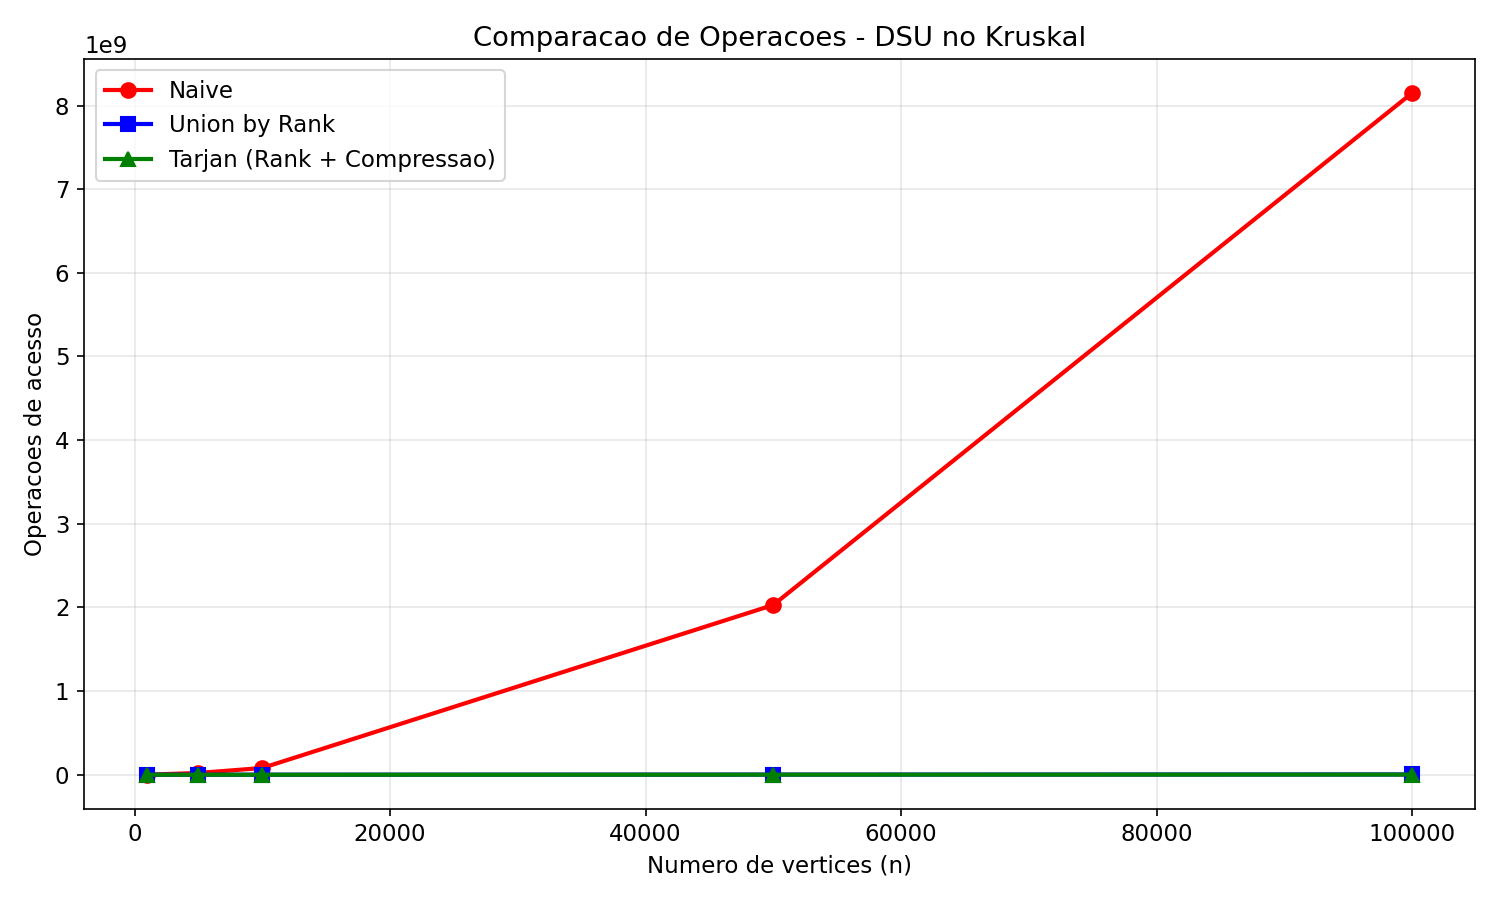
\includegraphics[width=0.85\textwidth]{grafico_operacoes_todas.png}
\caption{Comparação do número de operações entre as três variantes.}
\label{fig:ops_todas}
\end{figure}

A Figura~\ref{fig:ops_rank_tarjan} faz o zoom entre Rank e Tarjan. A compressão de caminho reduz o número de acessos em cerca de 34\% de forma consistente em todas as entradas testadas.

\begin{figure}[!ht]
\centering
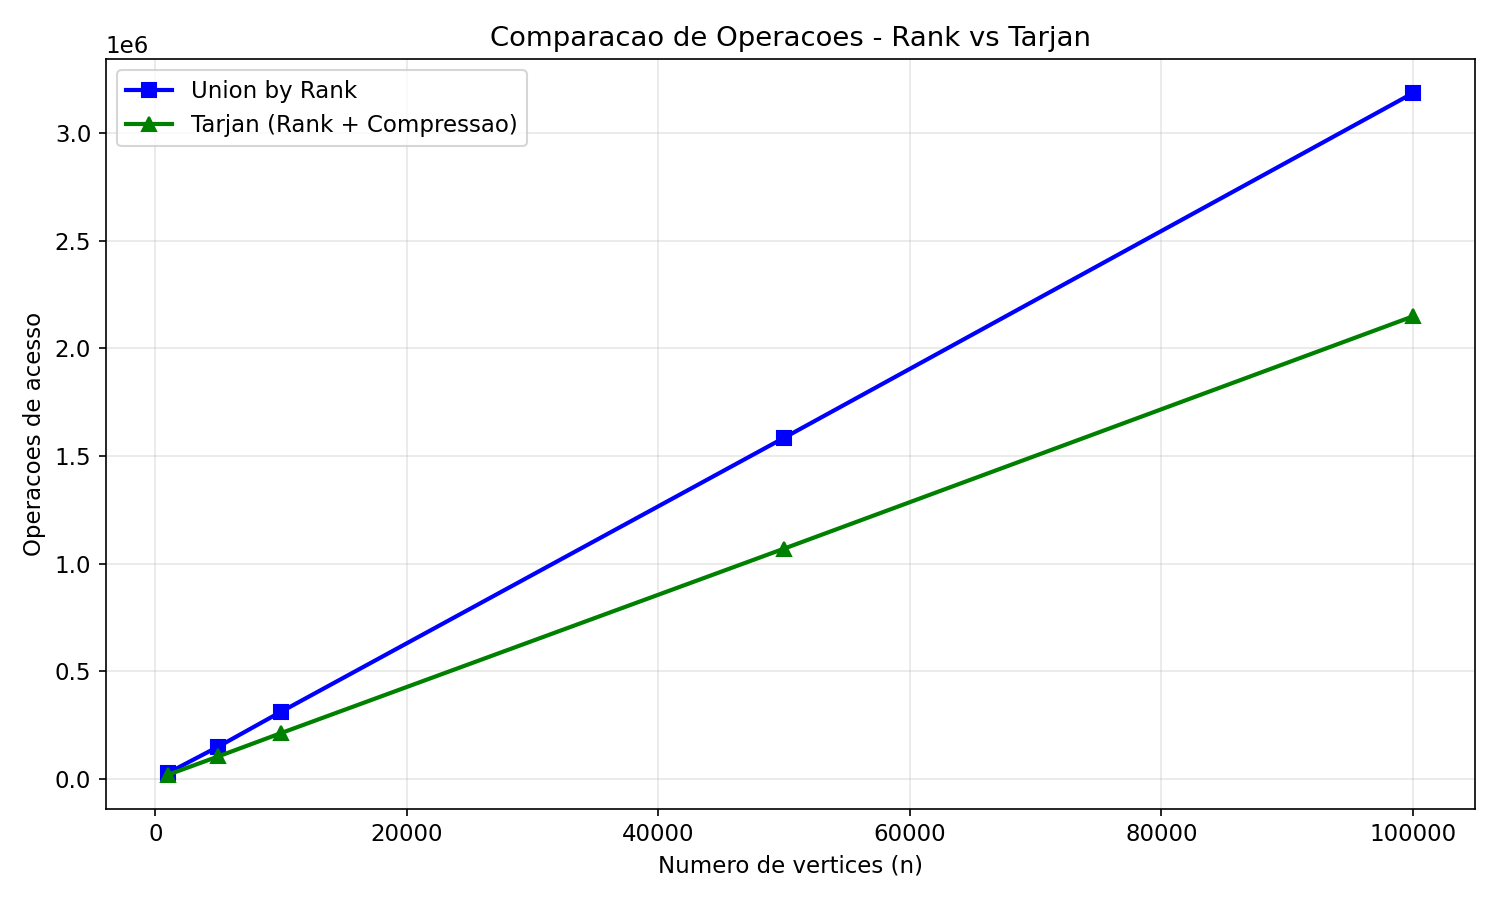
\includegraphics[width=0.85\textwidth]{grafico_operacoes_rank_tarjan.png}
\caption{Comparação de operações entre Union by Rank e Tarjan.}
\label{fig:ops_rank_tarjan}
\end{figure}

\subsection{Tempo de Execução}

A Tabela~\ref{tab:tempo} apresenta os tempos de execução medidos.

\begin{table}[!ht]
\centering
\caption{Tempo de execução em milissegundos (média $\pm$ desvio padrão amostral sobre 5 seeds)}
\label{tab:tempo}
\begin{tabular}{|r|r|r|r|}
\hline
\textbf{n} & \textbf{Naive (ms)} & \textbf{Rank (ms)} & \textbf{Tarjan (ms)} \\
\hline
1.000      & 1,28 $\pm$ 0,07        & 0,68 $\pm$ 0,11      & 0,58 $\pm$ 0,04    \\
5.000      & 13,94 $\pm$ 0,64       & 2,59 $\pm$ 0,10      & 2,39 $\pm$ 0,08    \\
10.000     & 50,92 $\pm$ 1,16       & 5,47 $\pm$ 0,14      & 5,04 $\pm$ 0,18    \\
50.000     & 3.392,31 $\pm$ 127,89  & 31,36 $\pm$ 2,59     & 29,07 $\pm$ 0,52   \\
100.000    & 16.235,40 $\pm$ 1.662,05 & 68,60 $\pm$ 2,73   & 63,17 $\pm$ 1,19   \\
\hline
\end{tabular}
\end{table}

Os tempos de execução, medidos após a fase de \textit{warm-up} do JIT, seguem a mesma hierarquia das contagens de acesso. Em $n = 10^5$, a versão Naive chega perto de 16,2 segundos, enquanto Rank e Tarjan ficam abaixo de 70 ms. A diferença passa de 230 vezes. Tarjan é mais rápido que Rank em todos os pontos testados; a vantagem é consistente, embora pequena em termos absolutos.

A Figura~\ref{fig:tempo_todas} evidencia essa disparidade em escala linear. A curva do Naive cresce de forma abrupta após $n = 10^4$, enquanto Rank e Tarjan permanecem praticamente sobrepostas à base do gráfico.

\begin{figure}[!ht]
\centering
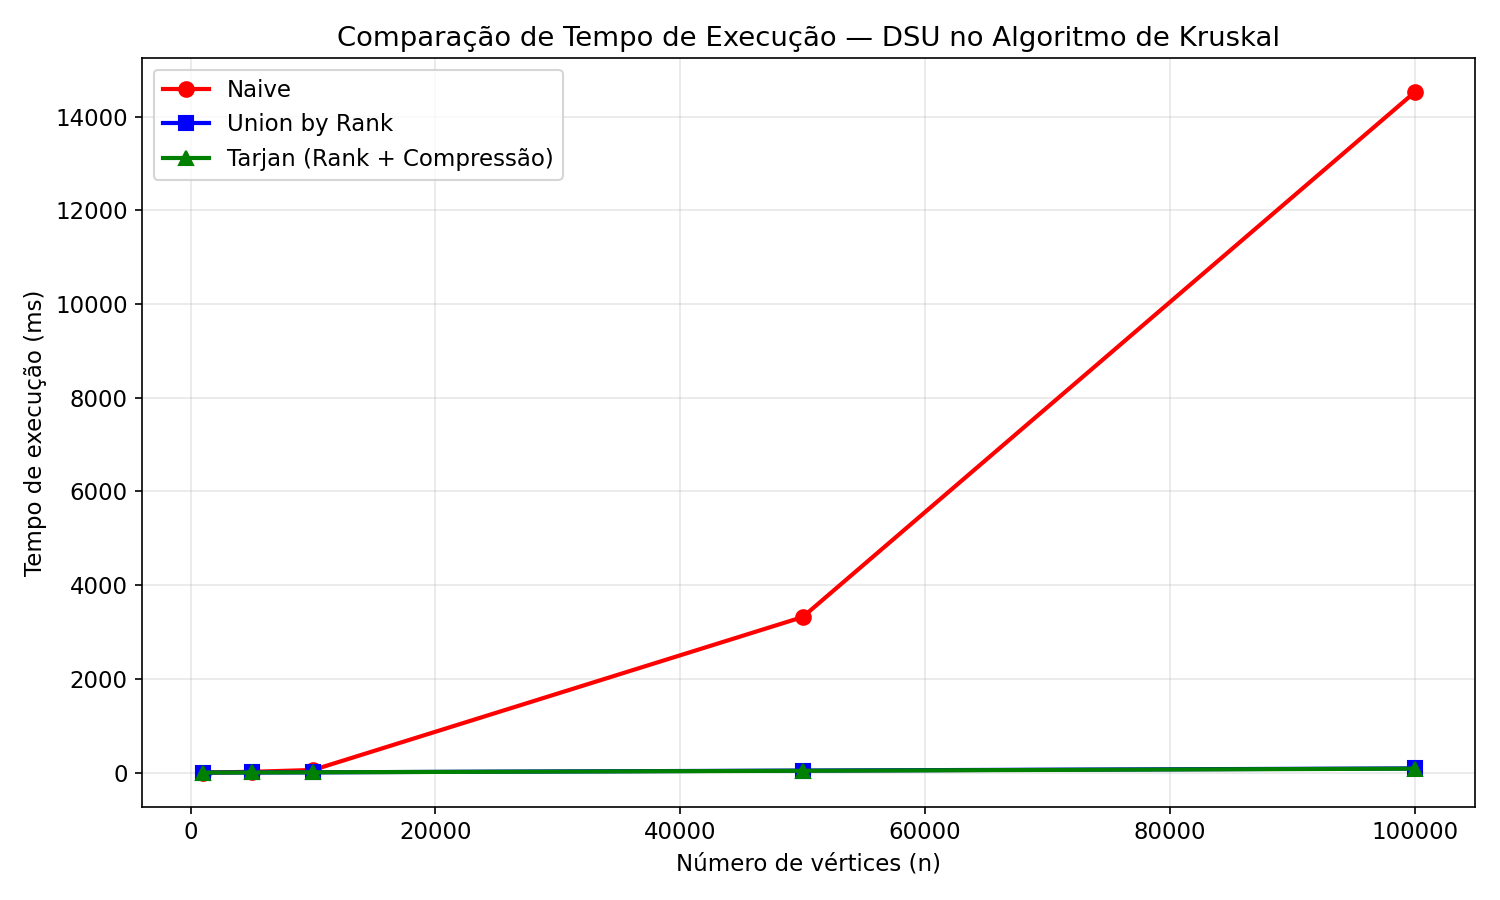
\includegraphics[width=0.85\textwidth]{grafico_tempo_todas.png}
\caption{Comparação de tempo de execução entre as três variantes.}
\label{fig:tempo_todas}
\end{figure}

Para isolar a diferença entre as duas variantes otimizadas, a Figura~\ref{fig:tempo_rank_tarjan} apresenta apenas Rank e Tarjan. Tarjan mantém vantagem consistente em todos os pontos, ainda que o ganho absoluto sobre Rank seja pequeno quando se considera o desvio padrão amostral.

\begin{figure}[!ht]
\centering
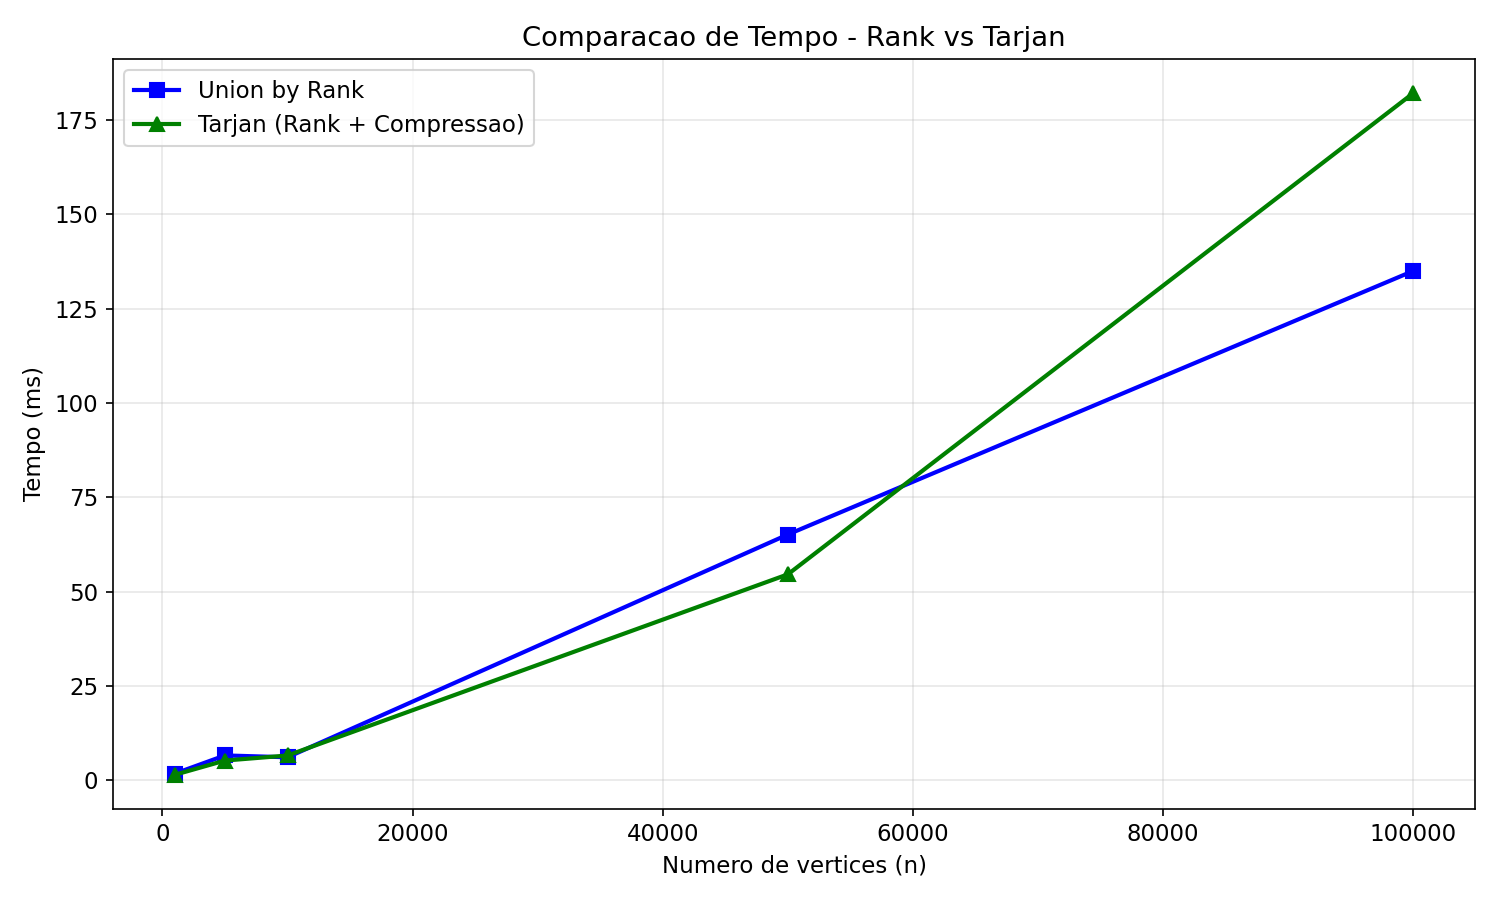
\includegraphics[width=0.85\textwidth]{grafico_tempo_rank_tarjan.png}
\caption{Comparação de tempo entre Union by Rank e Tarjan.}
\label{fig:tempo_rank_tarjan}
\end{figure}

\subsection{Classes de Complexidade e Custo Amortizado}

Para quantificar as classes de complexidade observadas experimentalmente, calcula-se o expoente empírico $p$ entre pares consecutivos de $n$, definido como $p = \log(\text{ops}_{i+1} / \text{ops}_i) / \log(n_{i+1} / n_i)$. Se o número de operações cresce como $n^p$, o valor de $p$ aproxima o expoente da classe de complexidade real. A Tabela~\ref{tab:expoente} apresenta os valores calculados.

\begin{table}[!ht]
\centering
\caption{Expoente empírico de crescimento das operações entre pares consecutivos de $n$ (médias sobre 5 seeds)}
\label{tab:expoente}
\begin{tabular}{|c|c|c|c|}
\hline
\textbf{Transição} & \textbf{Naive ($p$)} & \textbf{Rank ($p$)} & \textbf{Tarjan ($p$)} \\
\hline
$10^3 \to 5\cdot 10^3$     & 2,01 & 1,03 & 1,02 \\
$5\cdot 10^3 \to 10^4$     & 2,01 & 1,06 & 1,02 \\
$10^4 \to 5\cdot 10^4$     & 2,01 & 1,01 & 1,00 \\
$5\cdot 10^4 \to 10^5$     & 2,01 & 1,01 & 1,00 \\
\hline
\end{tabular}
\end{table}

O expoente do Naive se mantém em torno de 2 em todas as transições, confirmando o crescimento quadrático $O(n^2)$. Rank e Tarjan têm expoentes próximos de 1, o que é esperado: como $m = 3n$, o custo total de $O(m \log n)$ para Rank e $O(m \cdot \alpha(n))$ para Tarjan cresce essencialmente de forma linear em $n$, com o fator logarítmico ou de Ackermann contribuindo marginalmente. A Figura~\ref{fig:expoente} visualiza esse resultado.

\begin{figure}[!ht]
\centering
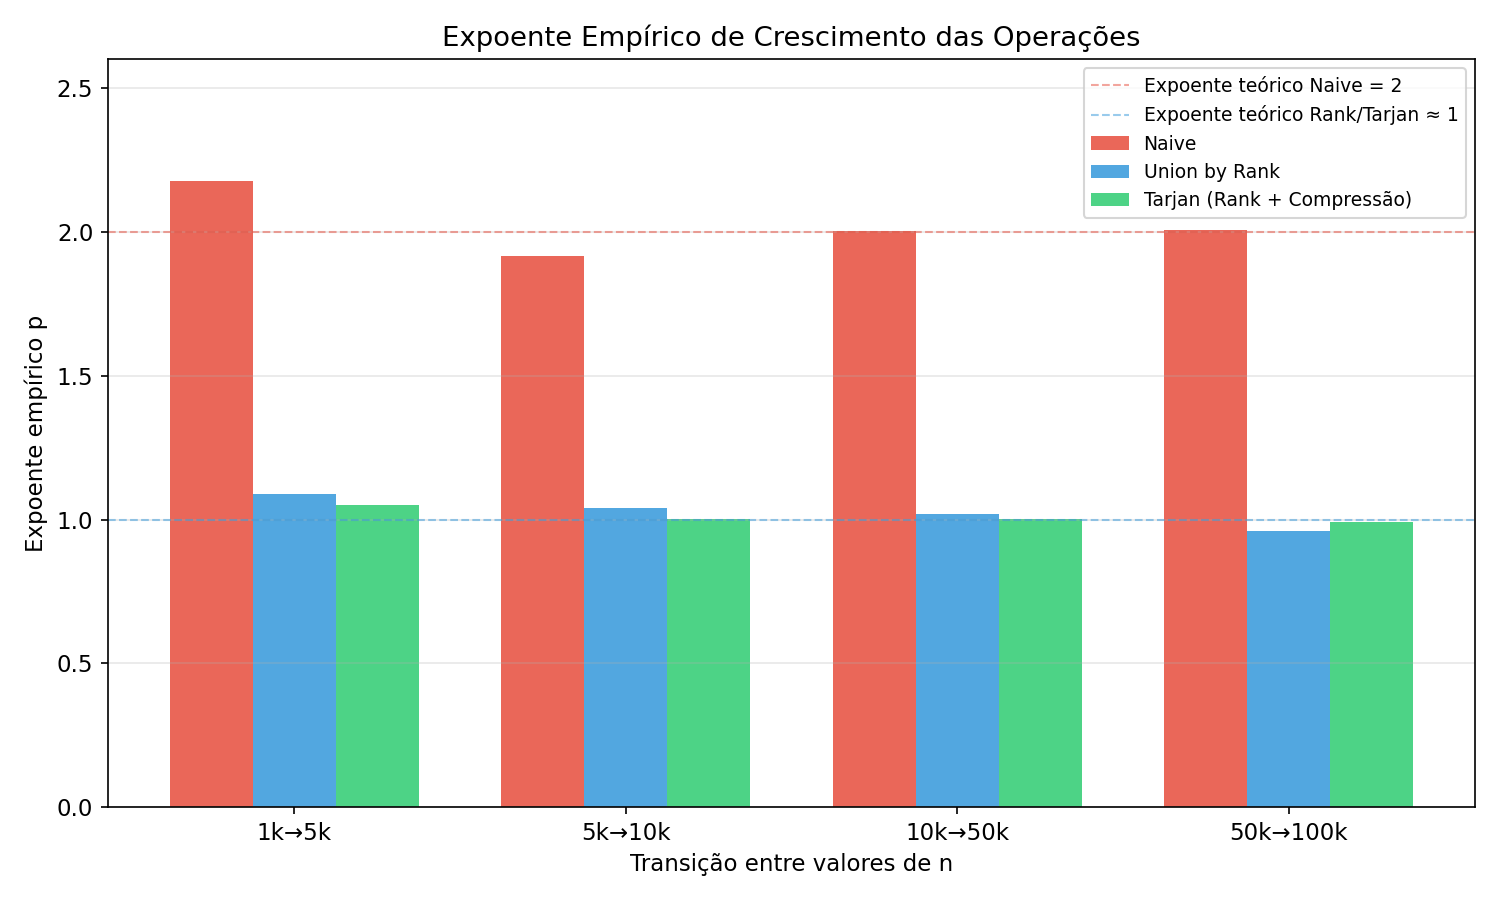
\includegraphics[width=0.85\textwidth]{grafico_expoente_empirico.png}
\caption{Expoente empírico de crescimento das operações por variante. Naive converge para 2 (quadrático); Rank e Tarjan ficam próximos de 1 (linear em $n$).}
\label{fig:expoente}
\end{figure}

A Figura~\ref{fig:log} usa escala logarítmica no eixo vertical. Nessa escala, curvas de classes diferentes exibem inclinações distintas, o que permite distinguir visualmente $O(n^2)$, $O(n \log n)$ e $O(n \cdot \alpha(n))$ sem ambiguidade. As três curvas têm inclinações claramente separadas, confirmando que as diferenças não são apenas de constante multiplicativa, mas de classe assintótica.

\begin{figure}[!ht]
\centering
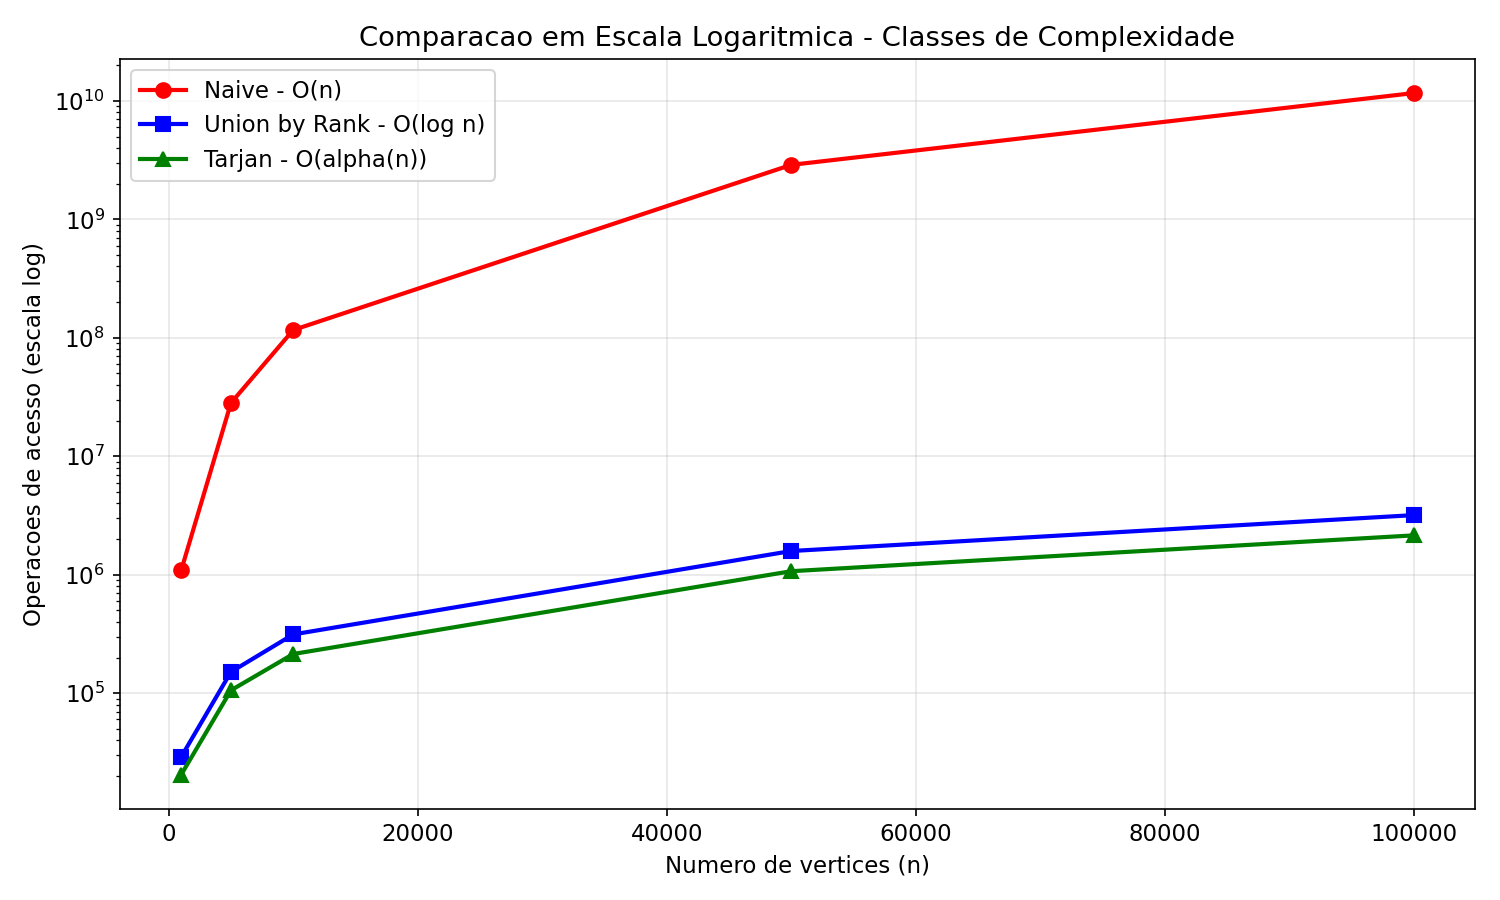
\includegraphics[width=0.85\textwidth]{grafico_log_operacoes.png}
\caption{Operações em escala logarítmica --- separação entre as classes de complexidade.}
\label{fig:log}
\end{figure}

A Figura~\ref{fig:custo_aresta} mostra o custo médio por aresta. No Naive, esse custo cresce linearmente com $n$, como seria de se esperar de operações $O(n)$. Rank apresenta crescimento lento, compatível com uma dependência logarítmica. Tarjan é o caso mais interessante: o custo por aresta fica praticamente plano ao longo de duas ordens de grandeza, e é essa estabilidade que corresponde, empiricamente, à complexidade amortizada $O(\alpha(n))$.

\begin{figure}[!ht]
\centering
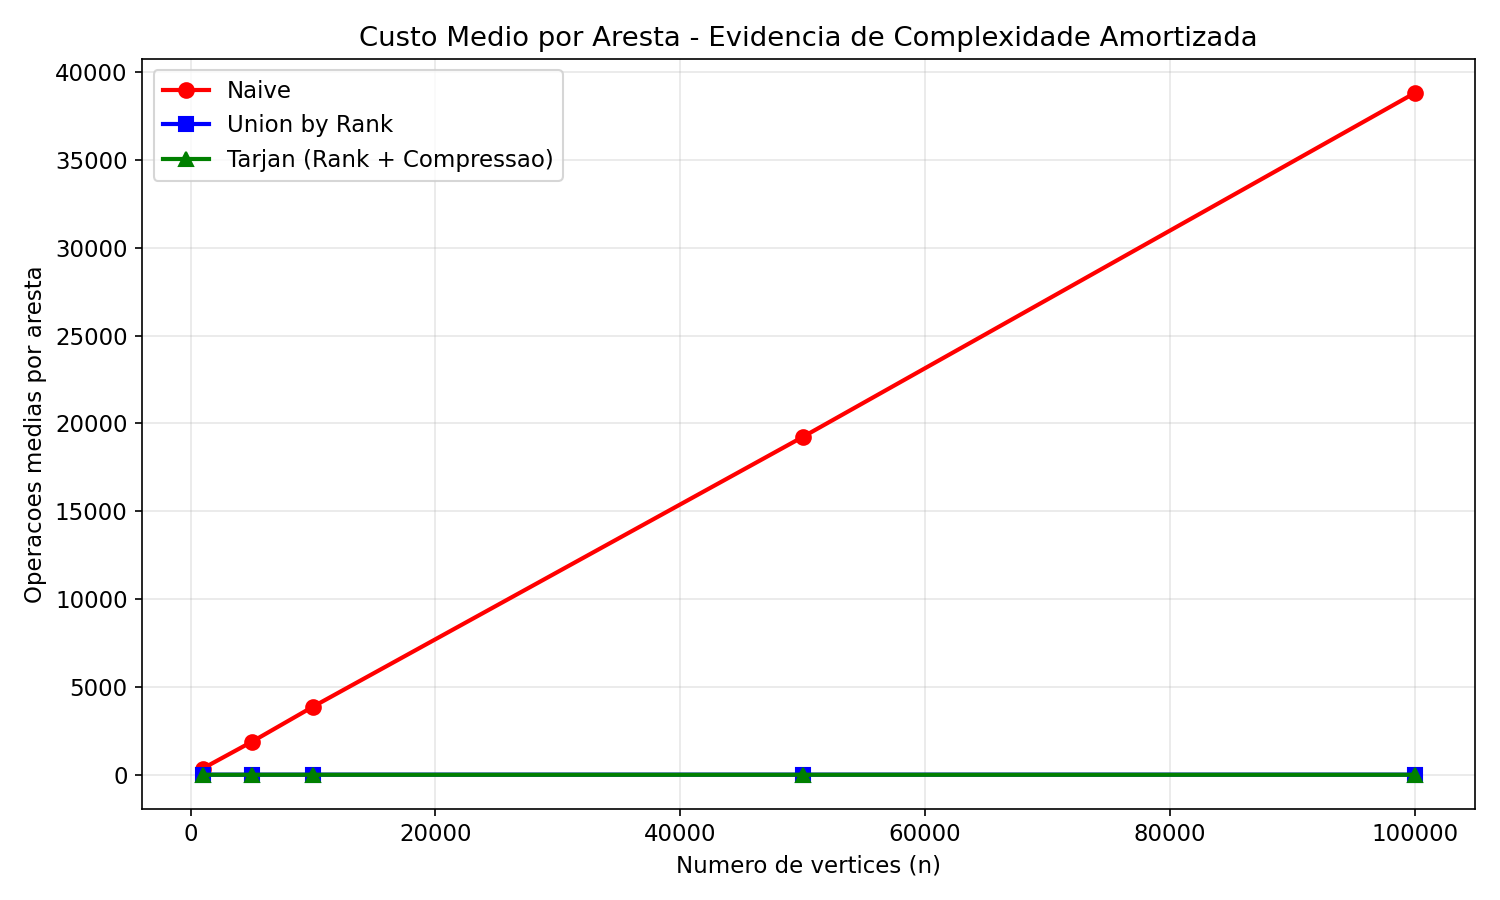
\includegraphics[width=0.85\textwidth]{grafico_custo_por_aresta.png}
\caption{Custo médio de operações por aresta --- evidência de complexidade amortizada.}
\label{fig:custo_aresta}
\end{figure}


\section{Conclusão}
\label{sec:conclusao}

A primeira pergunta da introdução era em que escala a implementação ingênua deixa de ser viável. Os experimentos respondem de forma bastante direta: já em $n = 10.000$, a versão Naive gasta perto de 51 ms, enquanto Rank e Tarjan ficam abaixo de 5,5 ms. Em $n = 10^5$, a diferença passa de 230 vezes no tempo e de 3.800 vezes no número de acessos. Para qualquer aplicação de MST em escala real, Naive é simplesmente inviável.

A segunda pergunta mirava o ganho marginal de acrescentar Path Compression ao Union by Rank. O resultado é positivo, mas mais modesto do que o passo anterior: a compressão reduz os acessos em cerca de 34\% e o tempo em torno de 8\% em $n = 10^5$. É suficiente para manter Tarjan consistentemente à frente de Rank, mas a conquista principal já havia sido feita pelo Union by Rank. Na prática, o que importa mais é que, com a estrutura completa de Tarjan, o custo do DSU deixa de dominar o Kruskal: o gargalo passa a ser a ordenação das arestas em $O(m \log m)$.

\subsection*{Limitações}

A topologia dos grafos gerados (árvore-caminho com arestas extras) não corresponde à distribuição uniforme de um grafo de Erd\H{o}s--R\'enyi, o que pode influenciar a profundidade média das árvores DSU. O intervalo de $n$ investigado vai até $10^5$; extrapolações para escalas maiores assumem que o regime assintótico já foi atingido no domínio medido. Os resultados devem ser lidos como evidência de tendências de complexidade, não como benchmarks absolutos de desempenho.

\subsection*{Trabalhos Futuros}

Uma continuação natural seria reimplementar o \texttt{find} de Tarjan de forma iterativa em dois passos (subida até a raiz seguida de compressão), eliminando o overhead de chamada recursiva e validando experimentalmente se o ganho de Tarjan sobre Rank se torna mais expressivo. Outras variantes de compressão, como \textit{path halving} (cada nó passa a apontar para o avô), também merecem comparação. Por fim, ampliar a escala para $n = 10^7$ e variar a densidade $m/n$ permitiria investigar como a topologia afeta o termo constante oculto em $O(\alpha(n))$.

\bibliographystyle{sbc}
\begin{thebibliography}{9}

\bibitem{tarjan1975}
Tarjan, R. E. (1975).
\newblock Efficiency of a Good But Not Linear Set Union Algorithm.
\newblock {\em Journal of the ACM}, 22(2):215--225.

\bibitem{tarjan1984}
Tarjan, R. E. and van Leeuwen, J. (1984).
\newblock Worst-case Analysis of Set Union Algorithms.
\newblock {\em Journal of the ACM}, 31(2):245--281.

\bibitem{tarjan1985}
Tarjan, R. E. (1985).
\newblock Amortized Computational Complexity.
\newblock {\em SIAM Journal on Algebraic and Discrete Methods}, 6(2):306--318.

\bibitem{kruskal1956}
Kruskal, J. B. (1956).
\newblock On the Shortest Spanning Subtree of a Graph and the Traveling Salesman Problem.
\newblock {\em Proceedings of the American Mathematical Society}, 7(1):48--50.

\bibitem{cormen2009}
Cormen, T. H., Leiserson, C. E., Rivest, R. L., and Stein, C. (2009).
\newblock {\em Introduction to Algorithms}. 3rd edition.
\newblock MIT Press.

\bibitem{sedgewick2011}
Sedgewick, R. and Wayne, K. (2011).
\newblock {\em Algorithms}. 4th edition.
\newblock Addison-Wesley.

\end{thebibliography}

\end{document}
